\subsection{Reverberation recordings in the elevator}

\begin{figure}[h]
\hspace*{3cm}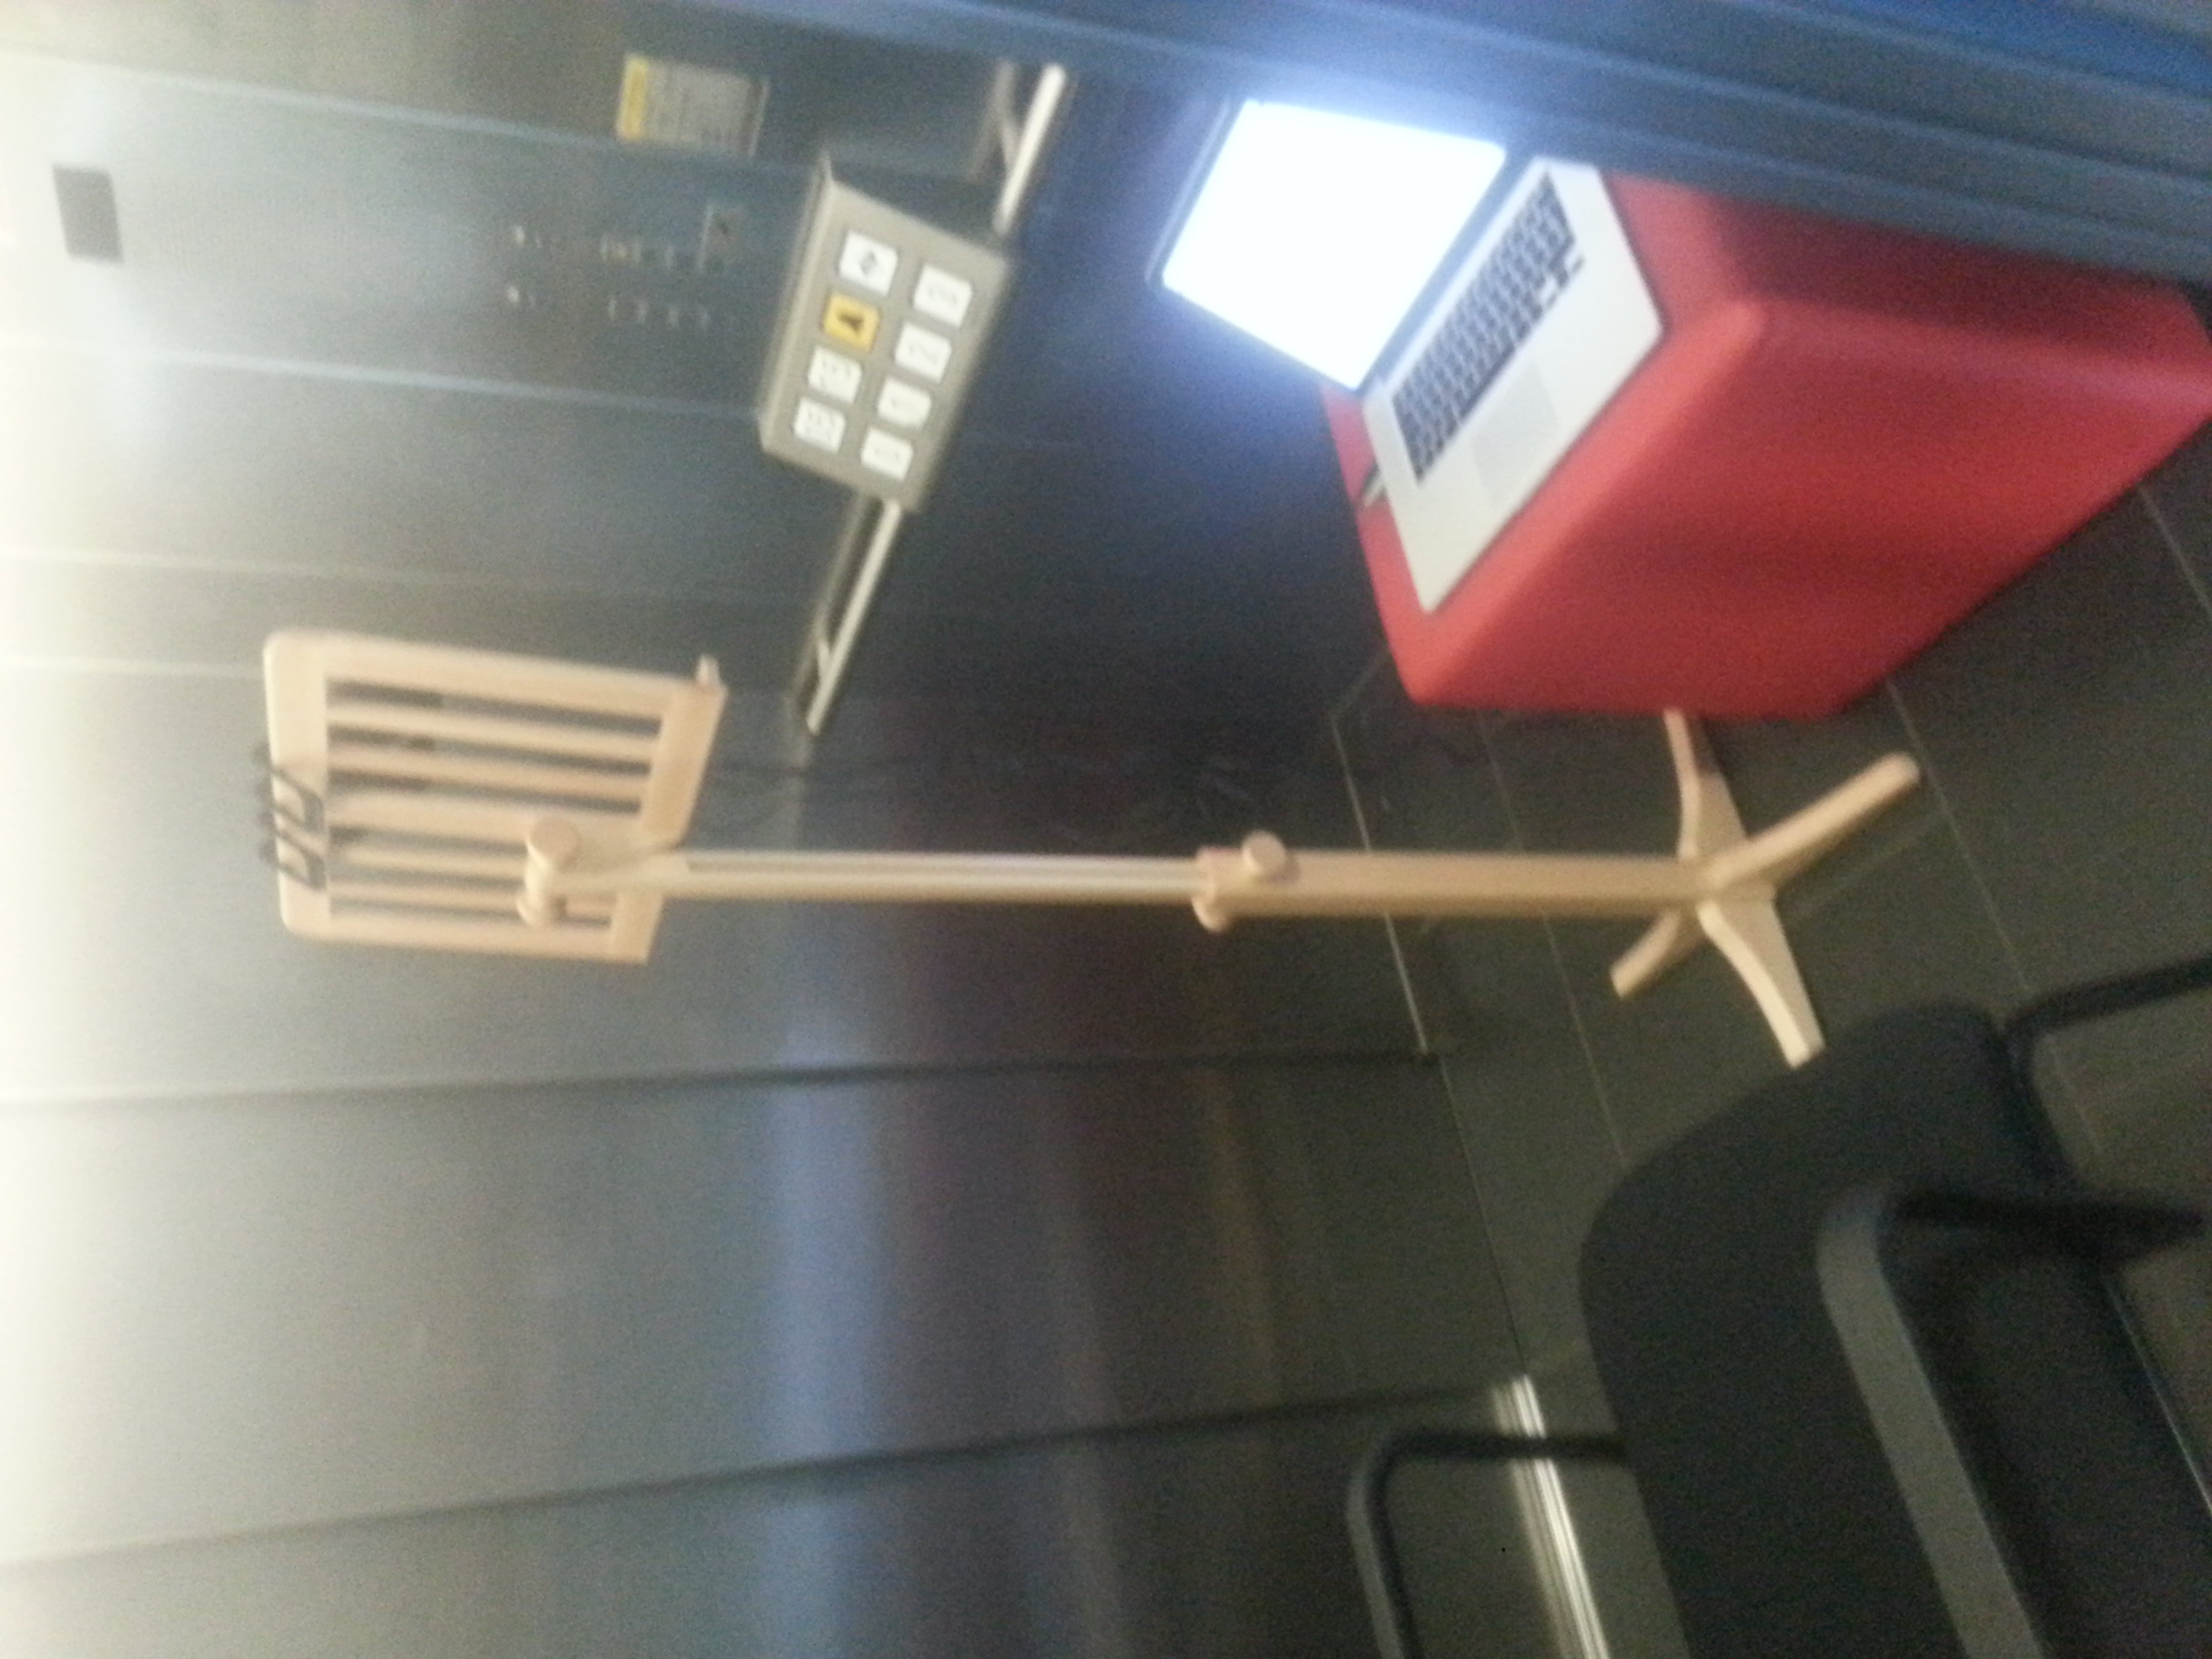
\includegraphics[scale=0.15]{setup_reverberation_rec.jpg}
\caption{Recordings setup.}
\label{fig:recordingsetup}
\end{figure}



\noindent To account for the noise of the elevator, its sound when moving, the sound of the doors opening and closing and the reverberation with open doors on the different floors and other noises from outside of the elevator, recordings were done via the elevator's built-in microphone. 
The setup used for this can be seen in picture \ref{fig:recordingsetup}.
It consisted of two loudspeakers positioned on a music stand at the height of approximately 150cm, at a distance of approximately 20cm from the elevator's microphone. 
The recordings made in the lab were played through the loudspeakers and recorded with Praat via the elevator's microphone. 
While the recordings were being played, the elevator was moved between the floors, its doors were opened and closed and kept with its doors opened and closed on different floors.

